\documentclass[11pt]{article}
\usepackage[margin=2.5cm]{geometry}
\usepackage{graphicx,booktabs,hyperref,amsmath}
\usepackage[T1]{fontenc}
\hypersetup{colorlinks=true,linkcolor=black,urlcolor=blue,citecolor=black}
\title{A systematic time error in the DASCH metadata of J.\,H.~Metcalf's early ``ma'' plates, and Pluto on four Harvard plates of 1908 and 1909}
\author{Qianghao Wu}
\date{November 24, 2026}
\begin{document}
\maketitle

\begin{abstract}
The DASCH exposure times of the early Harvard ``ma'' plates (J.\,H.~Metcalf, Taunton, 1905--1913) contain a systematic error. The error follows one rule with no free parameter: Metcalf's logged local mean time, counted from noon, was read as local sidereal time. The predicted shift is about $+6$\,h in December, about 0\,h in late March and about $\pm12$\,h in September. Five independent tests support the rule. (1) For 47 of 54 MPC observation times of Metcalf's own asteroids, the rule predicts the DASCH-minus-MPC offset within 1.5\,h; with the DASCH times taken as correct, 8 of 54 agree, and the best of 10{,}000 shuffles reaches 23 of 54. (2) Times printed by Metcalf in \emph{Astronomische Nachrichten}: 34 of 36 fit the rule and 0 of 36 fit the DASCH times. (3) For the lunar-eclipse plate ma00905 (1909 Nov 27), the DASCH midpoint is 2\,h before the penumbral eclipse began, and Metcalf's printed exposure matches totality to about 1\,min. (4) At the DASCH midpoints, 14 of 60 timed ma plates were exposed in daylight; after the correction, 1 of 60 is. (5) On four plates, a known asteroid is at its position for the corrected time and absent at its position for the DASCH time.
At the corrected times, a faint source is at Pluto's predicted position on ma00731 and ma00733 (1908 Dec 21, 22), more weakly on ma00729 (Dec 20), and on ma00937 (1909 Dec 12). The image on ma00731 was published first by Graham (2026), whose position agrees with ours to $0.2''$; the two analyses were made independently. The time-error rule, ma00733 and ma00937 are not in that paper. The identification is a candidate for expert examination of the glass plates.
\end{abstract}

\section{Relation to prior work}
Graham (2026, v1 published 2026 Nov 19) reports candidate images of Pluto on Harvard plate MA~731 (1908 Dec 21) and on two Heidelberg plates of 1909 Feb 20. Graham fits the exposure midpoint of MA~731 to the trail of (179)~Klytaemnestra and finds it 348\,min before the DASCH time. Graham takes the DASCH times to be local sidereal time, as the DASCH documentation states, and gives no cause for the offset on this plate.

This note was made independently. Its analysis started on 2026 Nov 17 (first commit \texttt{70df2ae}; the commit log is \texttt{GIT\_LOG.txt} in this record) and the author found Graham's paper on 2026 Nov 24. The results below that are not in Graham (2026) are:
\begin{enumerate}
\item the cause of the time offset and a correction rule for the whole early ma series, with tests on 54 MPC times, 36 printed times, an eclipse plate and the Sun altitude (Section~\ref{sec:time});
\item a signal at the corrected Pluto position on ma00733 ($z=+5.2$), a plate that Graham describes as ``neither supports nor contradicts'' the candidate;
\item a signal on ma00937 (1909 Dec 12), which is outside Graham's search window (which ends June 1909).
\end{enumerate}
Graham (2026, Appendix E) states that the cause of the MA~731 offset is not known. Graham tests one reading (a start time logged in sidereal time and read as mean time) and reports that it does not reproduce the archived time of MA~733. The rule in Section~\ref{sec:time} fits both plates.

ma00937 is not the earliest image of 1909. Wild et al.\ (1998) and Buchwald et al.\ (2000) reported Pluto on Barnard's Yerkes plates of 1909 Aug 20 and Nov 11; W.~Osborn and F.~Mills considered the November image ``fairly certain'' (Reichhardt 2015). Schaefer, Buie \& Smith (2008, Section~6) describe two earlier searches of the Harvard plates, in 1982 and 2004, which found no prediscovery image.

\paragraph{Heidelberg plates.} Before this note, the project measured the Heidelberg plates B2247a and B2248b (1909 Feb 20) under rules committed in advance (\texttt{archives/RULES.md}). The $z$ values at Pluto's position are $+5.47$ and $+6.42$; the pair gives $Z=+8.40$, and 13 of 2{,}000 control pairs reach that value. The rules classify the result as ``cannot measure'': at $3.5^\circ$ from the plate centre the image width is $20''$, and the position is on the wings of B 14--15 stars $29''$--$44''$ away. This result is consistent with Graham's images on these plates, but it does not confirm them. (Versions 1 and 2 of this note stated in error that the Heidelberg plates were not examined.)

\section{Data and method}
All plate data are public DASCH Data Release~7 cutouts (Grindlay et al.~2012), fetched one at a time through the public Starglass API (74 cutouts in total). Pluto and asteroid positions are JPL Horizons astrometric positions. Each cutout is reduced to a matched-filter significance map ($z$ map) with the plate's own point-spread width; catalog stars (Gaia DR3, APASS DR9) are masked. Significance in stacks is measured against 1{,}000 parallel and 1{,}000 scrambled control tracks. The pipeline was calibrated on 36 Harvard plates of the 1930s, where it recovers Pluto at SNR $+5.99$ (0 of 1{,}000 controls as high). For the on-plate asteroid test and the restack, the rules were committed to git before the relevant cutouts were fetched.

\section{The time error}\label{sec:time}
\subsection{Rule}
Let $t$ be the true time and $t_\mathrm{L}=\mathrm{LMT}(t)-12\,\mathrm{h} \pmod{24\,\mathrm{h}}$ the logged value: Taunton local mean time counted from noon. If DASCH read $t_\mathrm{L}$ as local sidereal time, the DASCH time $t_\mathrm{D}$ is the time nearest to $t$ with $\mathrm{LST}(t_\mathrm{D}) = t_\mathrm{L}$. The shift $t_\mathrm{D}-t$ depends only on the date. The rule has no free parameter. (Implementation: \texttt{timetest/match.py}, function \texttt{shift\_A}.)

\subsection{Tests}
\paragraph{MPC observations.} All MPC observations from Metcalf's own sites (Taunton 803, Winchester 799), 1905--1913, of his 41 asteroids and 2 comets, give 54 independent times that have an ma plate in DASCH whose field contains the MPC position. The rule predicts the DASCH-minus-MPC offset within 1.5\,h for 47 of 54 (median residual $-0.84$\,h). If the DASCH time were the true time, 8 of 54 would agree. When the predicted shifts are shuffled among the observations, the best of 10{,}000 shuffles reaches 23 of 54. With only one candidate plate per observation (no plate choice), 30 of 35 fit.

\paragraph{Times printed in \emph{Astronomische Nachrichten}.} Metcalf printed 36 independent times (Greenwich mean time from noon) between 1908 October and 1910 January (AN 182, 373; 183, 79; 183, 207; 183, 335; 184, 9; 184, 71). The printed-minus-DASCH offset agrees with the rule within 1.5\,h for 34 of 36, and with zero for 0 of 36. Thirty of the 36 times are not in the MPC data set.

\paragraph{Eclipse plate.} Metcalf photographed the total lunar eclipse of 1909 Nov 26/27 (AN 184, 9) with exposure 08:13:30--09:34:00 UT. Totality lasted from 08:13:55 to 09:35:04 UT1 (Espenak, EclipseWise). DASCH plate ma00905 has the same exposure length (80.5\,min), but its DASCH midpoint is 04:16:20 UT, before the penumbral eclipse began (06:13 UT). The DASCH time is wrong by $-4.62$\,h. This plate was exposed after local midnight. It fits the rule only if the log used a 12-hour clock after midnight; this variant was found after the eclipse result and rests on one plate.

\paragraph{Sun altitude.} At the DASCH midpoints, 14 of 60 timed ma plates (1905--1913) have the Sun above the horizon at Taunton. After the correction, 1 of 60 does (ma00165, which is also a misfit in the MPC test). For comparison, 0 of 159 plates of the Cambridge series ac, ai, am and i are in daylight.

\paragraph{On-plate asteroids.} On the four Pluto plates, a known asteroid ((179)~Klytaemnestra on ma00729, ma00731, ma00733; (464)~Megaira on ma00937) is on the plate. A trail filter along the asteroid's track gives $Z=+41$ to $+56$ at the corrected time and $Z=-0.6$ to $+0.4$ at the DASCH time (controls: maximum $+2.5$). The rules of this test were committed before the cutouts were fetched. All 4 plates pass. Table~\ref{tab:times} gives the measured trail centres.

\subsection{Limits}
Most residuals from the rule are at $-0.26$\,h, the difference between Eastern Standard Time and Taunton local mean time, or at $-0.26$\,h minus the exposure time. The cause is not known. About 1 plate in 8 does not follow the rule. There is no Metcalf observation between 1908 Oct 23 and 1909 Oct 17, so the 1908 December nights are tested only by the on-plate asteroids. The logbooks were not examined.

A side finding: the MPC times of (694) and (695) on 1909 Nov 8 are 4\,h\,44\,min later than the times printed in AN 183, 79. This is the longitude of Taunton. With the printed times, both observations fit the rule.

\section{Pluto on ma00729, ma00731, ma00733 and ma00937}
At the DASCH times, nothing is at Pluto's predicted position on these plates ($z=-0.8$ to $+1.5$). A point source is $16''$--$19''$ east of that position on each plate, mostly along Pluto's track. This offset equals a plate time 5.4--6.6\,h earlier than the DASCH time. At the plate times measured from the asteroid trails, Pluto's Horizons position is $1.3''$, $1.2''$ and $0.1''$ from the source on ma00729, ma00731 and ma00937, and $3.4''$ on ma00733, where the offset is across the track (Table~\ref{tab:times}). Graham (2026) also reports on MA~733 an excess $3''$--$4''$ from the prediction, mostly across the track. (Versions 1 and 2 of this note gave the along-track component only and stated in error that all four distances are within $1.0''$.)

\begin{table}[h]
\centering\footnotesize\setlength{\tabcolsep}{4pt}
\begin{tabular}{lllllcl}
\toprule
Plate & Night & DASCH (UT) & Trail (UT) & Source (J2000) & $z$ & Pluto--source (along, across)\\
\midrule
ma00729 & 1908 Dec 20 & 06:56 & 00:58 & 05 43 39.4 \ +16 00 59 & $+2.0$ & $1.3''$ ($-1.0''$, $+0.8''$)\\
ma00731 & 1908 Dec 21 & 06:46 & 01:05 & 05 43 34.5 \ +16 01 00 & $+7.5$ & $1.2''$ ($-1.2''$, $+0.3''$)\\
ma00733 & 1908 Dec 22 & 06:49 & 01:17 & 05 43 29.5 \ +16 00 58 & $+5.2$ & $3.4''$ ($-0.1''$, $-3.4''$)\\
ma00937 & 1909 Dec 12 & 07:35 & 01:11 & 05 48 38.3 \ +16 19 49 & $+6.5$ & $0.1''$ ($-0.1''$, $+0.1''$)\\
\bottomrule
\end{tabular}
\caption{Plate times and the Pluto candidate. ``DASCH'': archived midpoint. ``Trail'': midpoint measured from the asteroid trail. $z$: peak value. ``Pluto--source'' is the distance between Pluto's Horizons position at the trail time and the source, with its components along and across Pluto's motion.}\label{tab:times}
\end{table}

\paragraph{Checks.}
\begin{itemize}
\item The source moves with Pluto: at the sky position of one night's source, the other nights show $z=-0.6$ to $+1.1$.
\item Catalogs (Gaia DR3 and Pan-STARRS1 DR2, all magnitudes, within $12''$): no Gaia source is within $9.9''$ of any source position. The nearest Pan-STARRS1 objects are $r=21.7$ at $10.3''$ (ma00729), $r=21.2$ at $8.8''$ (ma00731), $r=20.2$ at $7.0''$ (ma00733) and $r=20.9$, $g=21.6$ at $3.1''$ (ma00937). The candidate has $B\approx16.3$, so a cataloged object at these positions would need an outburst of more than 4 mag. The ma00731 values agree with Graham (2026).
\item On ma00731, Graham's image centre (RA $85.893708^\circ$, Dec $+16.016635^\circ$) is $0.19''$ from the source position in Table~\ref{tab:times}. Graham's trail-fit midpoint (00:58:24 UT) differs from ours by 7\,min; Pluto moves about $0.2''$ in that time.
\item Restack: with the rules fixed in advance and only the ma times corrected, all 20 pre-1910 plates give SNR $+8.15$ (parallel controls) and $+11.48$ (scrambled controls). Without the four candidate plates, the remaining 16 plates (none of them ma plates) give $+3.60$ and $+4.72$. This is not an independent detection at $5\sigma$. At the uncorrected DASCH times, all 20 plates give $+2.21$.
\item Look-elsewhere estimate: the chance that two unrelated peaks as strong as those on ma00731 and ma00733 fall as close together in the search disc is about $3\times10^{-6}$ to $6\times10^{-5}$. For ma00937, which was examined after the 1908 offset was known, it is about $2\times10^{-3}$. These are estimates from small counts.
\end{itemize}

\paragraph{Limits.} The four plates were inspected before the restack rules were written. ma00729 is shallower (limit 15.5) and its signal is weak. The scans cannot exclude an emulsion flaw, a transient, or an asteroid that is unknown today. Examination of ma00731 and ma00733 under a loupe, and Metcalf's logbook entries for these nights, would test both the time rule and the candidate directly. Barnard's Yerkes 10-inch Bruce plates 10B-501, 502, 505 and 506 (1908 Dec 19--28) cover Pluto's position on nights near the Harvard plates and would give an independent check.

\section*{Changes in version 3}
Corrected the distances between Pluto and the source (Section~4, Table~\ref{tab:times}); corrected the statement about the Heidelberg plates; added the prior Yerkes and Harvard work; added the Pan-STARRS1 catalog check.

\section*{Data and code}
The project repository is included in this record (\texttt{pluto-dasch-code.zip}): all code, the cutout manifest with SHA-256 hashes and request payloads, the MPC and AN tables, and all result files. The FITS cutouts are not included; the manifest gives the requests that fetch them again from the public DASCH API.

\section*{AI disclosure}
The analysis, the code and the text were produced with AI coding agents (Anthropic's Claude) under the author's direction. The work has not been reviewed by experts.

\section*{Acknowledgments}
This work has made use of data provided by Digital Access to a Sky Century @ Harvard (DASCH), which has been partially supported by NSF grants AST-0407380, AST-0909073, and AST-1313370. Work on DASCH Data Release 7 received support from the Smithsonian American Women's History Initiative Pool. This work used JPL Horizons, the Minor Planet Center observation database, Gaia DR3, APASS DR9 and Pan-STARRS1 DR2 through VizieR, the Heidelberg Digital Plate Archive, and the NASA ADS scans of \emph{Astronomische Nachrichten}.

\section*{References}
\begin{itemize}\setlength\itemsep{0pt}
\item Buchwald, G., DiMario, M. \& Wild, W. 2000, ASP Conf.\ Ser.\ 220, 355
\item Graham, P. 2026, Candidate images of Pluto on archival plates from 1908 and 1909, Zenodo, \href{https://doi.org/10.5281/zenodo.24376800}{doi:10.5281/zenodo.24376800}
\item Grindlay, J. et al. 2012, IAU Symposium 285, 29 (2012IAUS..285...29G)
\item Metcalf, J.\,H. 1909--1910, Astronomische Nachrichten 182, 373; 183, 79; 183, 207; 183, 335; 184, 9; 184, 71
\item Reichhardt, T. 2015, Air \& Space Magazine, July 15
\item Schaefer, B.\,E., Buie, M.\,W. \& Smith, L.\,T. 2008, Icarus 197, 590
\item Wild, W.\,J., Buchwald, G., DiMario, M.\,J. \& Standish, E.\,M. 1998, BAAS 30 (DPS), 55.14
\item Espenak, F., EclipseWise, Total lunar eclipse of 1909 Nov 27, \url{https://eclipsewise.com/lunar/LEprime/1901-2000/LE1909Nov27Tprime.html}
\end{itemize}

\appendix
\section{Figures}
\begin{figure}[h]
\centering
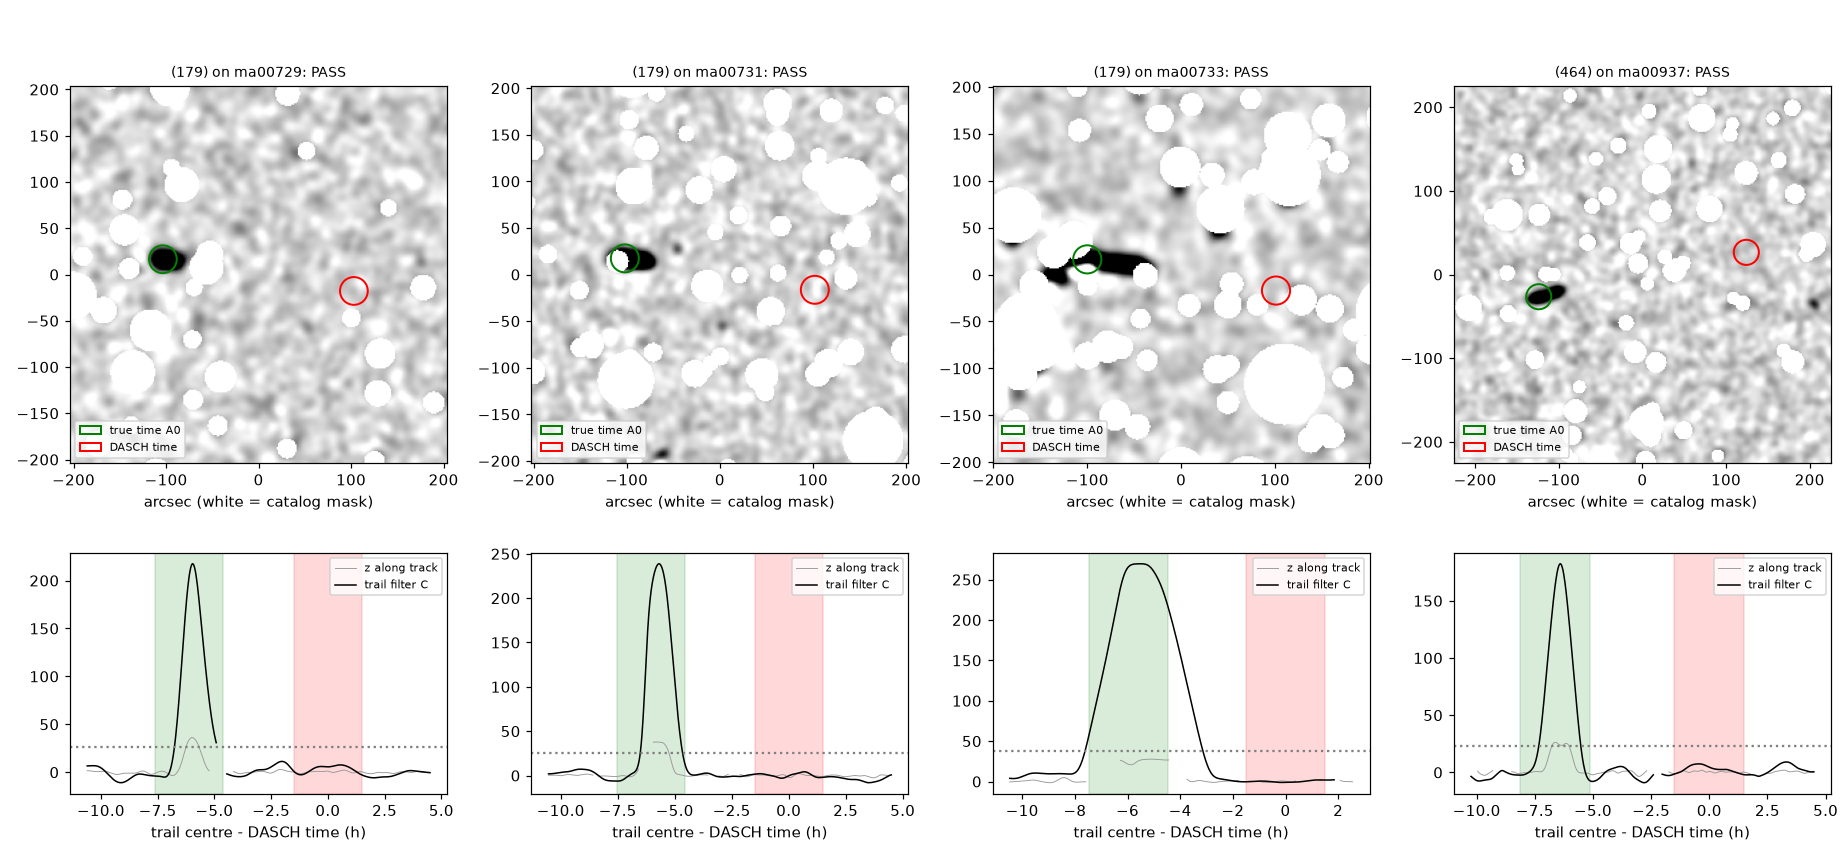
\includegraphics[width=\textwidth]{figures/stamps.png}
\caption{On-plate asteroid test. Top: $z$ maps; green: asteroid position at the corrected time; red: at the DASCH time. Bottom: $z$ and trail filter along the track.}
\end{figure}
\begin{figure}[h]
\centering
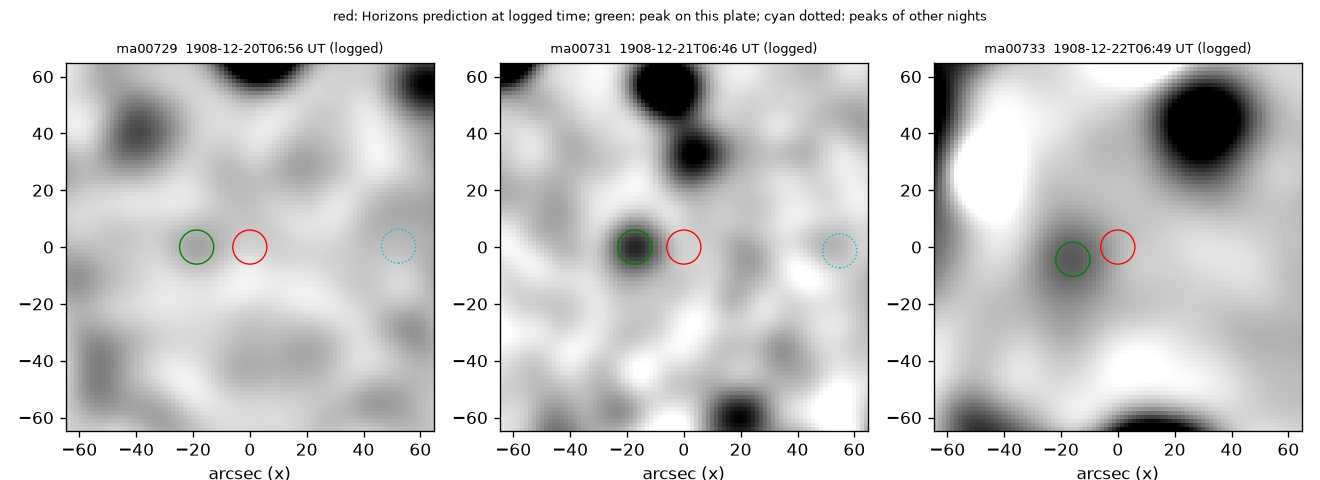
\includegraphics[width=\textwidth]{figures/candidate_1908.png}
\caption{The candidate on the three 1908 plates ($z$ maps). Red: Pluto's position at the DASCH time; green: the peak on this plate; cyan, dotted: the peaks of the other nights.}
\end{figure}
\end{document}
